\section{Identidad del proyecto: naming y diseño del logotipo}
\label{sec:identidad_proyecto}

Antes de iniciar la fase de codificación, resultó fundamental dotar al proyecto de una identidad verbal y visual coherente que sintetizara la propuesta de valor del sistema. La plataforma no debía percibirse como un mero portal transaccional de clasificados inmobiliarios, sino como un ecosistema integral pensado para facilitar la experiencia completa de habitar un piso compartido.

Inicialmente se exploraron diversas propuestas de denominación centradas de forma exclusiva en la búsqueda de alojamiento estudiantil (nombres provisionales como \emph{UniRooms}, \emph{FlatStudent} o \emph{PisoShare}). Sin embargo, estas alternativas se descartaron con rapidez por resultar excesivamente asépticas, impersonales y reduccionistas: omitían por completo el núcleo diferencial del software, que radica en la convivencia comunitaria cotidiana, el reparto equitativo de tareas y la gestión transparente de gastos entre compañeros.

Con el objetivo de reflejar adecuadamente la filosofía del \emph{co-living} universitario, se abordó un proceso de búsqueda que fusionara dos conceptos angulares:
\begin{itemize}
    \item El prefijo \textbf{``Co''}, derivado directo de \emph{co-living}, \emph{comunidad} y \emph{convivencia cooperativa}.
    \item La raíz verbal y fonética \textbf{``livi''}, procedente del término inglés \emph{living} (vivir, habitar, vida compartida).
\end{itemize}

De esta simbiosis léxica surgió la denominación definitiva: \textbf{Colivi}. Se trata de un nombre breve, eufónico y memorable, dotado de un carácter contemporáneo que comunica de inmediato la misión del proyecto: ``convivir y vivir juntos de forma sencilla y transparente''.

A partir de esta identidad verbal se concibió el diseño del logotipo corporativo, alineado con las especificaciones del sistema de diseño descritas en el capítulo anterior. Se persiguió una composición sobria y reconocible que integrara un isotipo geométrico representativo y el logotipo tipográfico. El isotipo estiliza la silueta protectora de un tejado y los pilares del hogar, entrelazando elementos que simbolizan la convergencia armónica de distintos miembros bajo un mismo espacio residencial. 

En cuanto a la armonía cromática, se aplicó rigurosamente la paleta maestra: el tono terracota cálido (\#C85A32) como color primario de marca —que transmite calidez de hogar, energía y hospitalidad— combinado con el azul marino profundo (\#0F172A) para la marca tipográfica, proyectando solidez estructural y rigor técnico.

El resultado final de esta identidad visual se exhibe a continuación en la figura \ref{fig:logo_colivi}.

\begin{figure}[H]
    \centering
    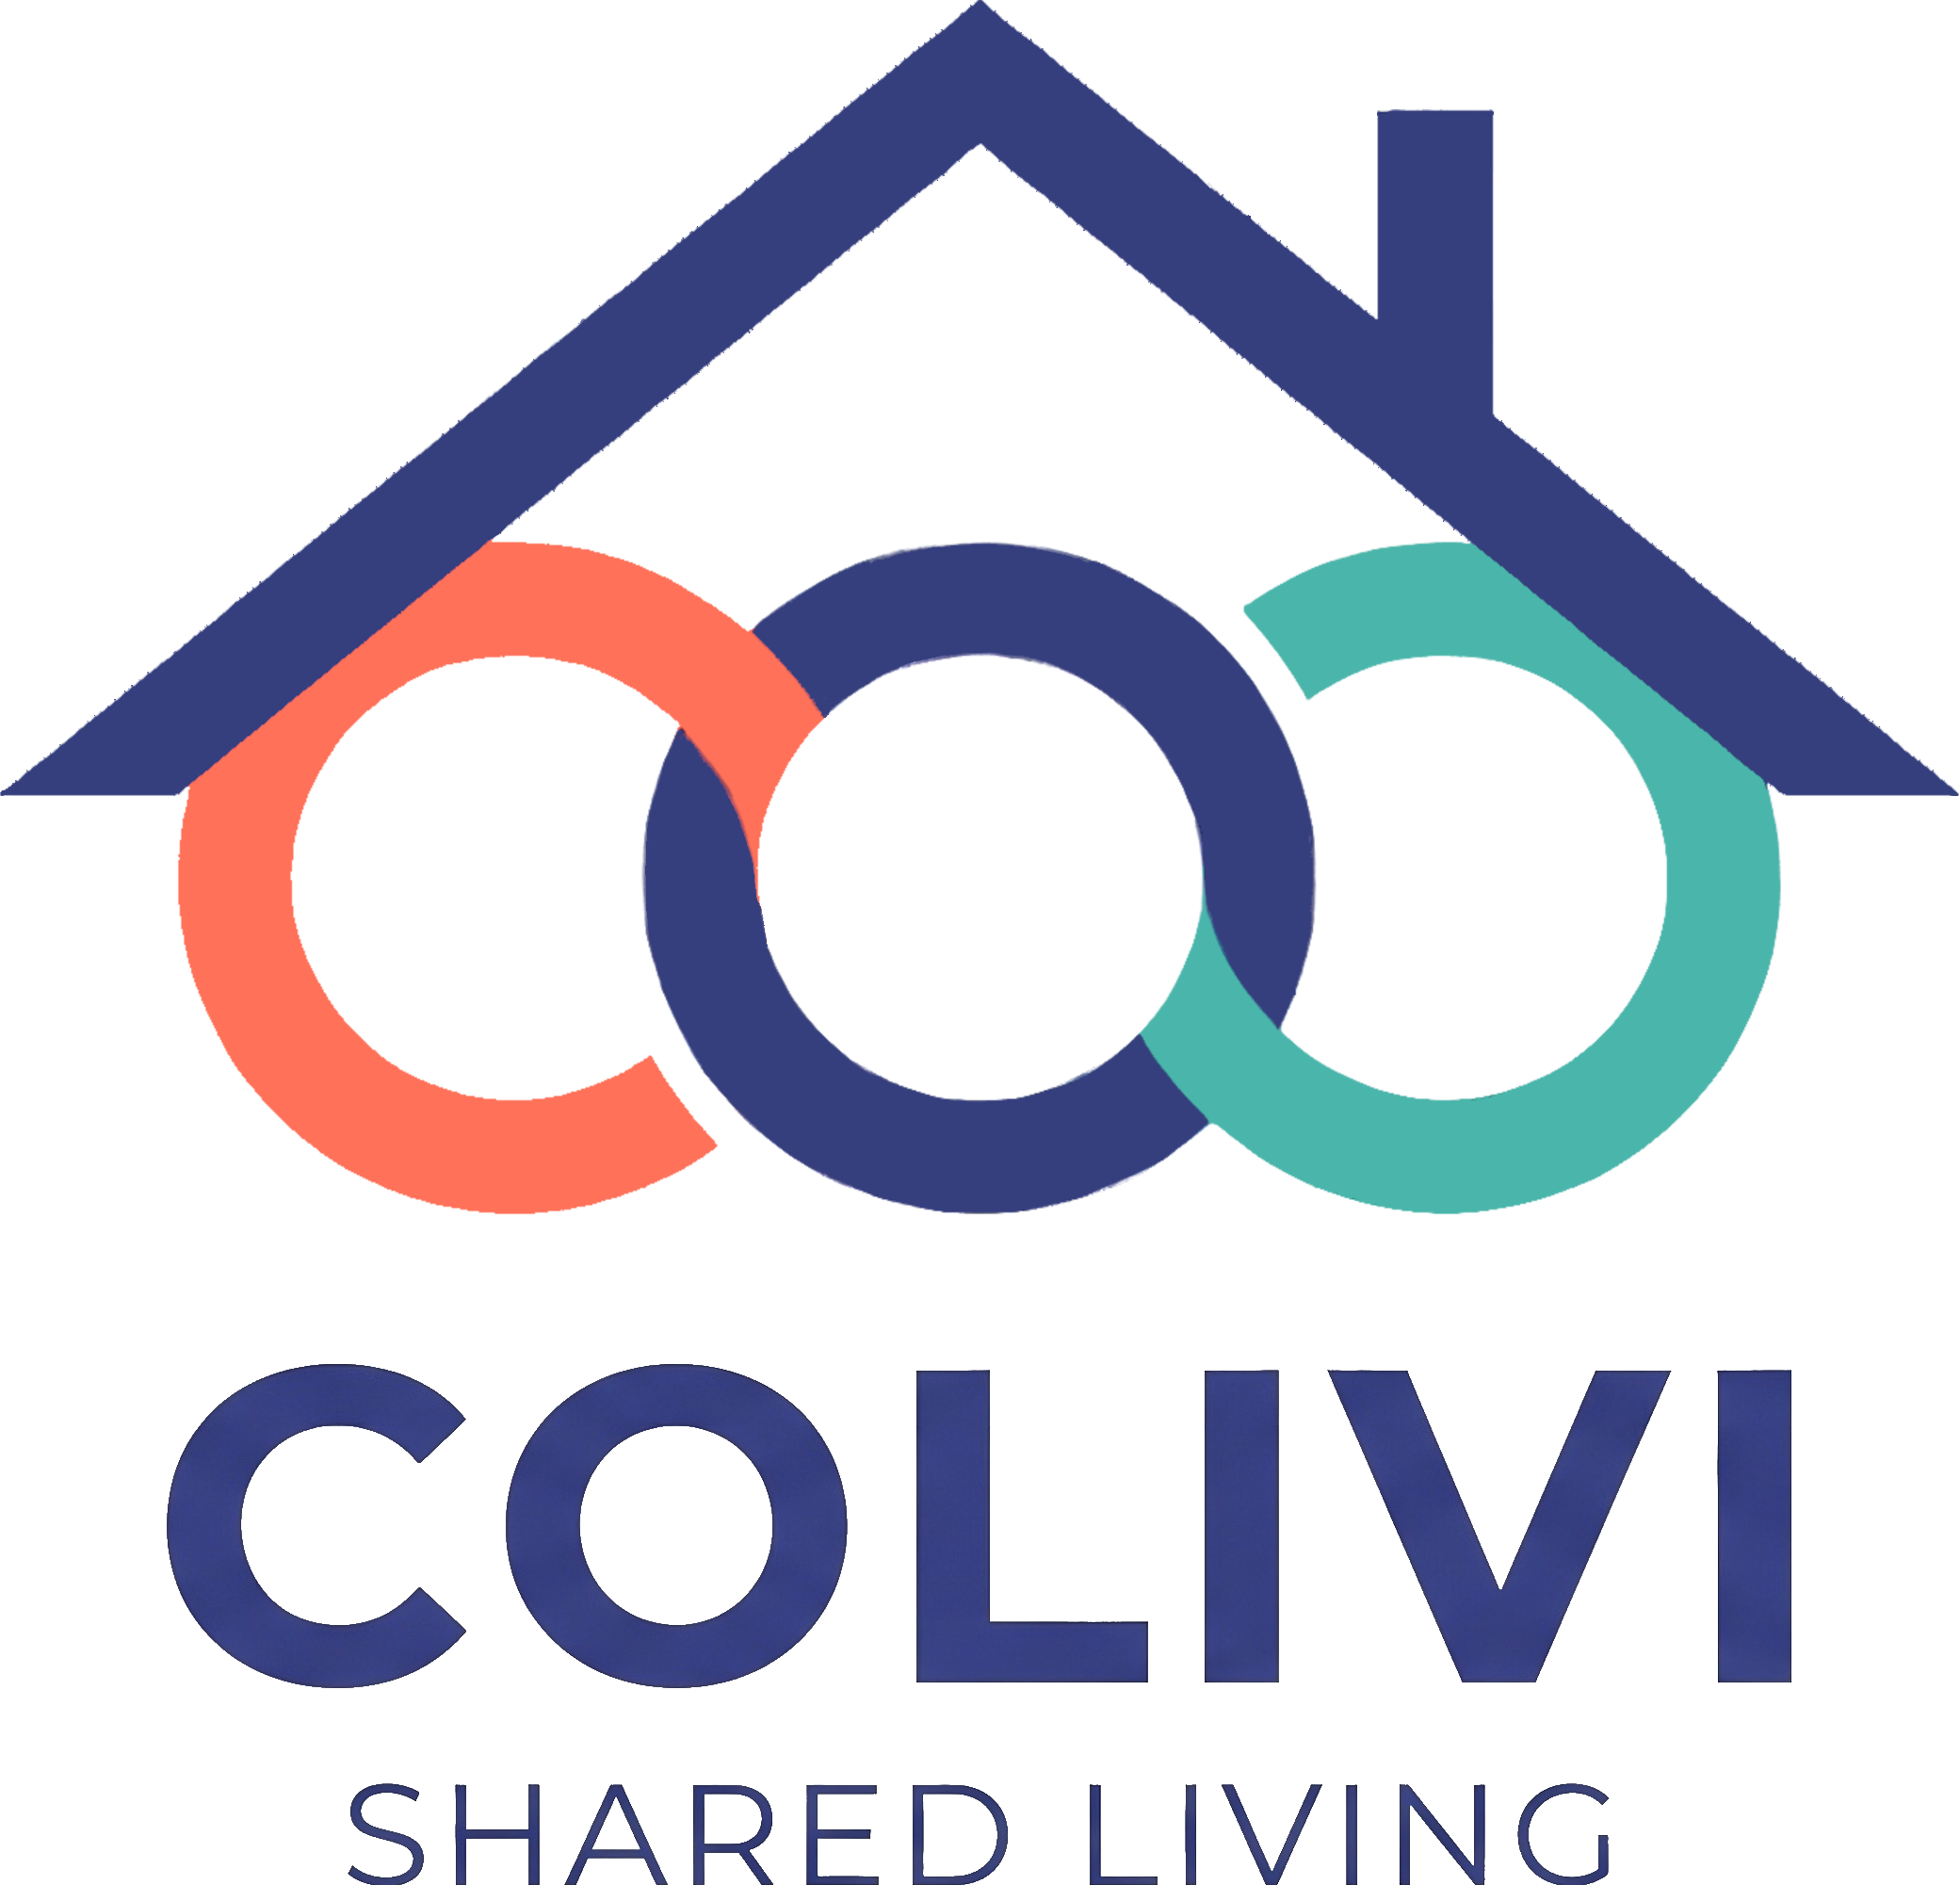
\includegraphics[width=0.45\textwidth]{DesarrolloDeColivi/img/logo_colivi.png}
    \caption{Logotipo corporativo e imagotipo oficial de Colivi.}
    \label{fig:logo_colivi}
\end{figure}

